\chapter{Często popełniane błędy}

\subsection*{Znaki pisarskie --- kreski poziome}

Należy poprawnie stosować znaki: ,,-'', ,,--'', ,,---'' oraz ,,$-$''. Po szczegóły odsyłam do Wikipedii.

\subsection*{Akapity}

Bezwzględnie nie należy używać polecenia
\begin{verbatim}
    \\
\end{verbatim}
do tworzenia nowego akapitu. Polecenie to właściwie nie powinno być wcale używane, poza szczególnymi przypadkami.

Nowy akapit tworzymy przez pozostawienie pustej linii w kodzie, lub za pomocą polecenia
\begin{verbatim}
    \par
\end{verbatim}
Aby usunąć wcięcie akapitowe używamy polecenia
\begin{verbatim}
    \noindent
\end{verbatim}
natomiast aby wymusić wcięcie również dla pierwszego akapitu, dodajemy paczkę
\begin{verbatim}
    \usepackage{indentfirst}
\end{verbatim}
do nagłówka.
Akapit powinien składać się z co najmniej dwóch zdań i trzech linii.

\subsection*{Rysunki, listingi i inne floaty}

Każdy float powinien być podpisany. Do floata odwołujemy się wyłącznie poprzez mechanizm referencji. Dzięki temu pozycja floata względem tekstu którego dotyczy nie jest istotna. W tekście musi znajdować się odwołanie do \textbf{każdego} floata. Jeżeli nie jesteśmy wyłącznymi autorami floata, bezwzględnie zaznaczamy jego źródło. Przykładowe metody załączania źródło pokazano na rysunkach \ref{fig:koty1} i \ref{fig:koty2}.

\begin{figure}
    \centering
    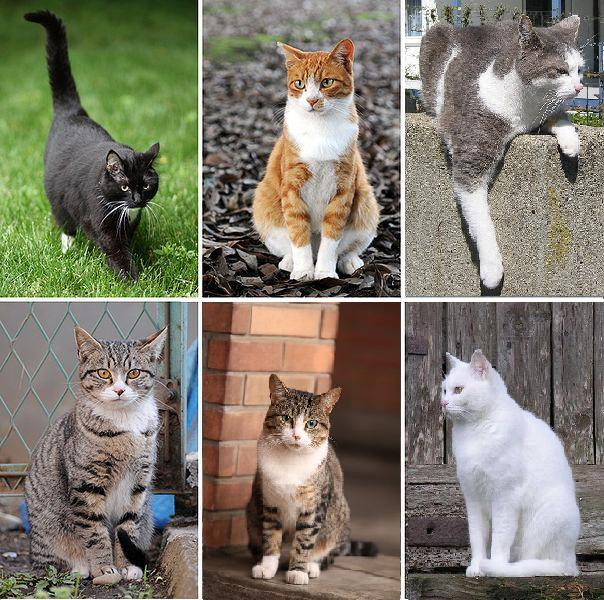
\includegraphics[width=.5\textwidth]{chapters/mistakes/img/kot1.jpg}
    \caption{To są koty z Internetu}%
    \label{fig:koty1}
    \footnotesize{źródło: Wikipedia, autor nieznany, na licencji CC, dostęp \today \\ \url{https://commons.wikimedia.org/wiki/File:Collage_of_Six_Cats-03.JPG}}
\end{figure}

\begin{figure}
    \centering
    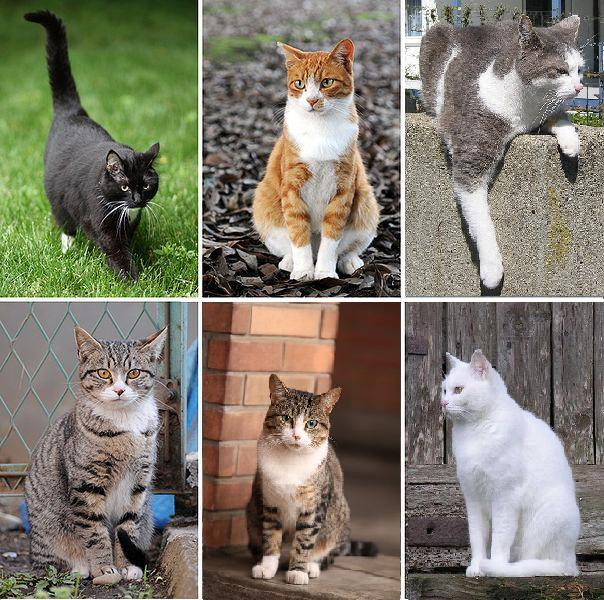
\includegraphics[width=.5\textwidth]{chapters/mistakes/img/kot1.jpg}
    \caption{To są koty z Internetu}%
    \label{fig:koty2}
    \footnotesize{źródło: Wikipedia \cite{kot1}}
\end{figure}
